\documentclass{article}
\usepackage{ketpic,ketlayer}
\usepackage{amsmath,amssymb}
\usepackage{graphicx}
\usepackage{xcolor}
\usepackage{bm,enumerate}
\usepackage[colorlinks=true,urlcolor=blue]{hyperref}

\setmargin{20}{20}{16}{20}

\renewcommand{\labelitemi}{$\cdot$}

\pagestyle{empty}

\begin{document}

\begin{center}
installing of KeTCindy 
\end{center}

\hfill Modified\ :\ \today

\begin{enumerate}[\bf\large 1.]
\item Install Cinderella, R, Maxima (and Sumatra only for Windows)
 \begin{itemize}
 \item \url{https://beta.cinderella.de}  (Cinderella)
 \item \url{https://cran.r-project.org}   (R)
 \item \url{https://sourceforge.net/projects/maxima/files}  (Maxima)
 \item \url{https://www.sumatrapdfreader.org/download-free-pdf-viewer.html} (Sumatra)
 \end{itemize}
\item Install TeX if any TeX has not been installed.
 \begin{enumerate}[(1)]
 \item TeXLive is recommended.
    \begin{itemize}
    \item KeTCindy has been implemented (2018 or later).
    \end{itemize}
 \item KeTTeX is a light-weight TeXLive.
    \begin{itemize}
    \item Download from\\
    \hspace*{5mm}Mac (kettex.dmg)\\
    \hspace*{10mm}\url{https://www.dropbox.com/s/dc4inuk06t07g26/kettex.dmg?dl=0}\\
    \hspace*{5mm}Windows (kettex.exe)\\
    \hspace*{10mm}\url{https://www.dropbox.com/s/fthw4btjqqs33tc/kettex.exe?dl=0}\\
    \hspace*{5mm}Linux (kettex.tar.xz)\\
    \hspace*{10mm}\url{https://www.dropbox.com/s/vg8p07832e9hzlk/KeTTeX-linux-20171022.tar.xz?dl=0}
     \item Move kettex generated by double clicking to the folder as follows.\\
     \hspace*{10mm}Mac\ \ /Applications,Windows\ \ C:\
    \end{itemize}
 \end{enumerate}

\item Install KeTCindy
  \begin{enumerate}[(1)]
  \item Download ketcindy from CTAN(\url{https://ctan.org}).\\
  \hspace*{10mm}Search ketcindy $>$ Pack­age ketcindy $>$ download\ (ketcindy)
    \begin{itemize}
    \item[Rem)]The latest version is downloadable from Repository:\\
         \hspace*{5mm}Clone or download $>$ Download ZIP\ (ketcindy-master)
    \end{itemize}
  \item Double click \verb|ketcindysettings.cdy| in the folder.
    \begin{itemize}
    \item Set Cinderella as the executive program if necessary.
   \item The figure may not appear at first.
   \end{itemize}

\vspace{2mm}

\begin{layer}{140}{0}
\putnotese{27}{20}{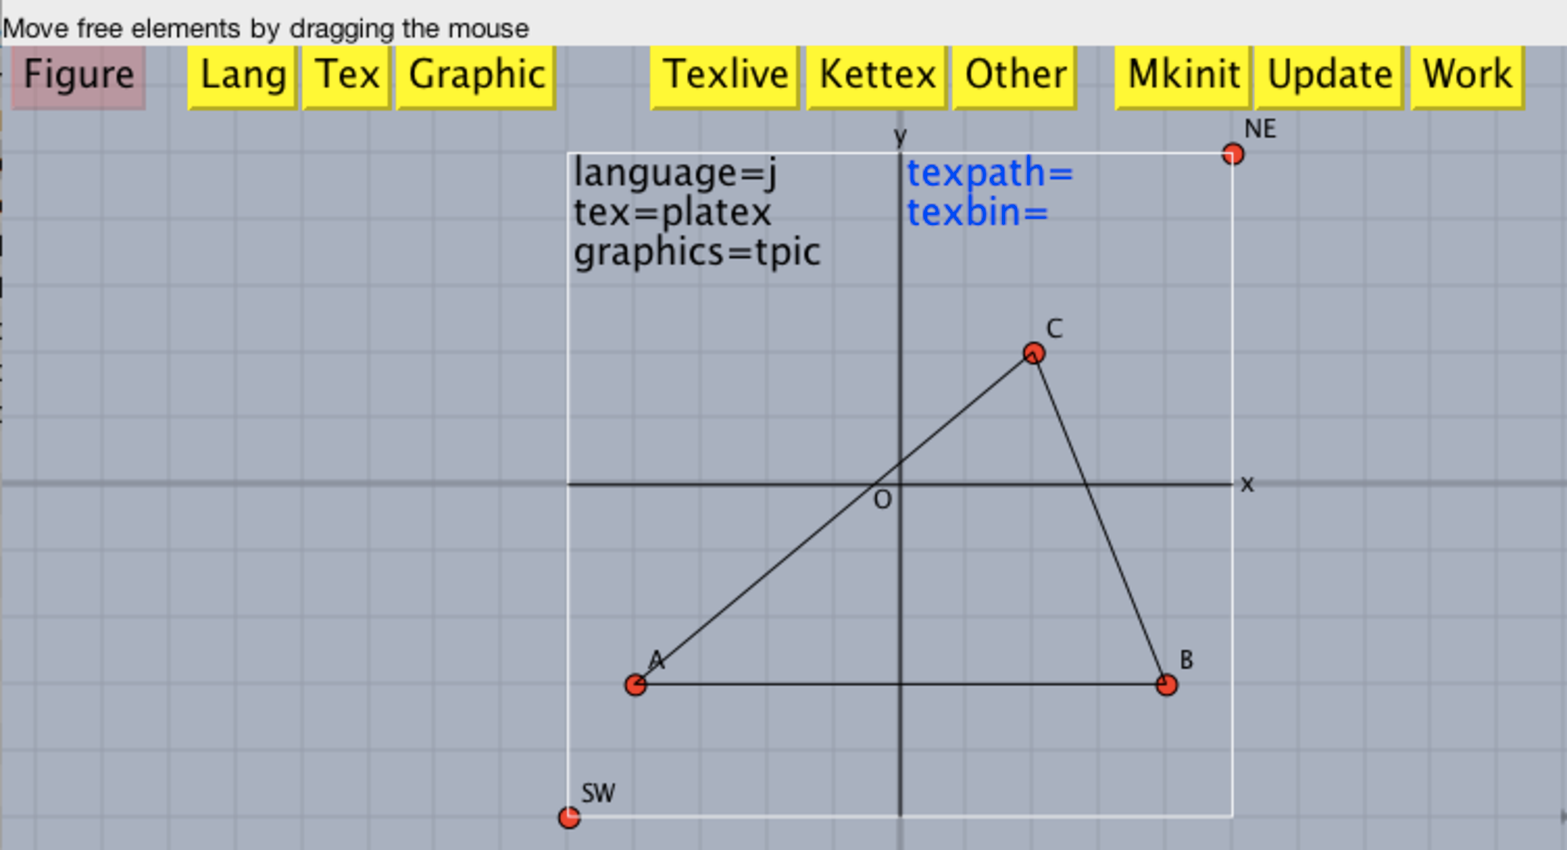
\includegraphics[bb=0.00 0.00 752.00 408.00,width=100mm]{Fig/setting.pdf}}
\putnotee{0}{5}{\bf [1]\ Select language,etc}
\putnotese{3}{10}{\underline{Language}}
\putnotese{7}{15}{Japanese, English}
\putnotese{3}{20}{\underline{\TeX}}
\putnotese{5}{24}{\begin{tabular}{l}
platex\\uplatex\\latex\\xelatex\\pdflatex\\lualatex\end{tabular}}
\putnotese{3}{51}{\underline{Graphic Code}}
\putnotese{5}{55}{\begin{tabular}{l}tpic\\pict2e\\tikz\end{tabular}}
\arrowline{47}{20}{17}{135}
\putnoten{83}{7}{\bf [2]Select \TeX\ sytem}
\arrowline{83}{20}{13}{90}
\putnotee{125}{5}{\bf [3]\ Folder operation}
\arrowline{110}{20}{20}{45}
\putnotese{131}{10}{\begin{minipage}[t]{30mm}%
\underline{Mkinit}\\
\hspace*{2mm}Create the init file\\
\hspace*{6mm}'ketcindy.ini'\\
\hspace*{2mm}in user's home.\\
\underline{Update}\\
\hspace*{2mm}Update ketcindy\\
\underline{Work}\\
\hspace*{2mm}Create work folder\\
\hspace*{6mm}'ketcindy'\\
\hspace*{2mm}in user's home.\\
\hspace*{2mm}Manuals, samples\\
\hspace*{2mm}will be included.
\end{minipage}}
\end{layer}

\vspace{77mm}

{\bf [4]\ Test run}\\
\hspace*{10mm}Press \verb|Figure| button, and the pdf will be displayed.

  \end{enumerate}

  \end{enumerate}

\end{document}